% =============================================================
\chapter{การพัฒนาระบบและผลการทดลอง}
\label{ch:results}
% =============================================================

\section{การพัฒนาส่วนติดต่อผู้ใช้}

รูปที่ \ref{fig:ui_showcase} แสดงหน้าจอหลักของระบบ ภาพทั้งหมดอยู่ใน \texttt{docs/01\_Reports/images/useindoc/}

\begin{figure}[H]
\centering
\begin{subfigure}[b]{0.48\textwidth}
    
\includegraphics[width=\textwidth]{images/useindoc/01_game_hub_before_login.png}
    \caption{หน้าแรก (Game Hub)}
\end{subfigure}
\hfill
\begin{subfigure}[b]{0.48\textwidth}
    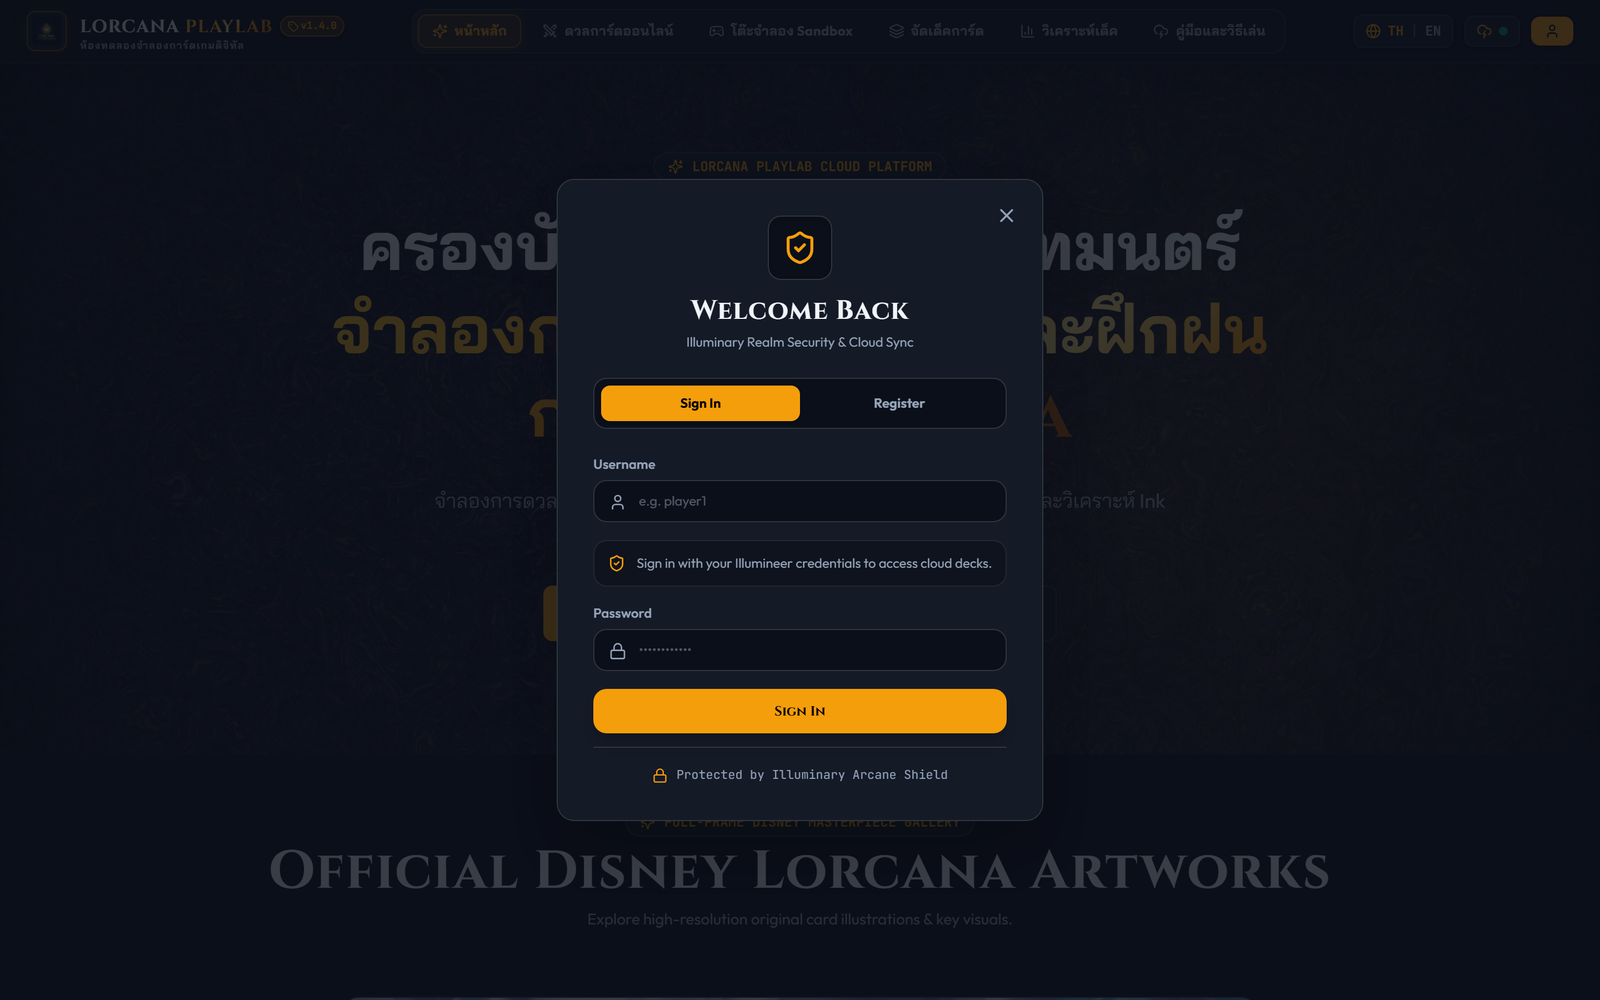
\includegraphics[width=\textwidth]{images/useindoc/02_login_modal.png}
    \caption{หน้าต่างเข้าสู่ระบบ}
\end{subfigure}
\\[0.3cm]
\begin{subfigure}[b]{0.48\textwidth}
    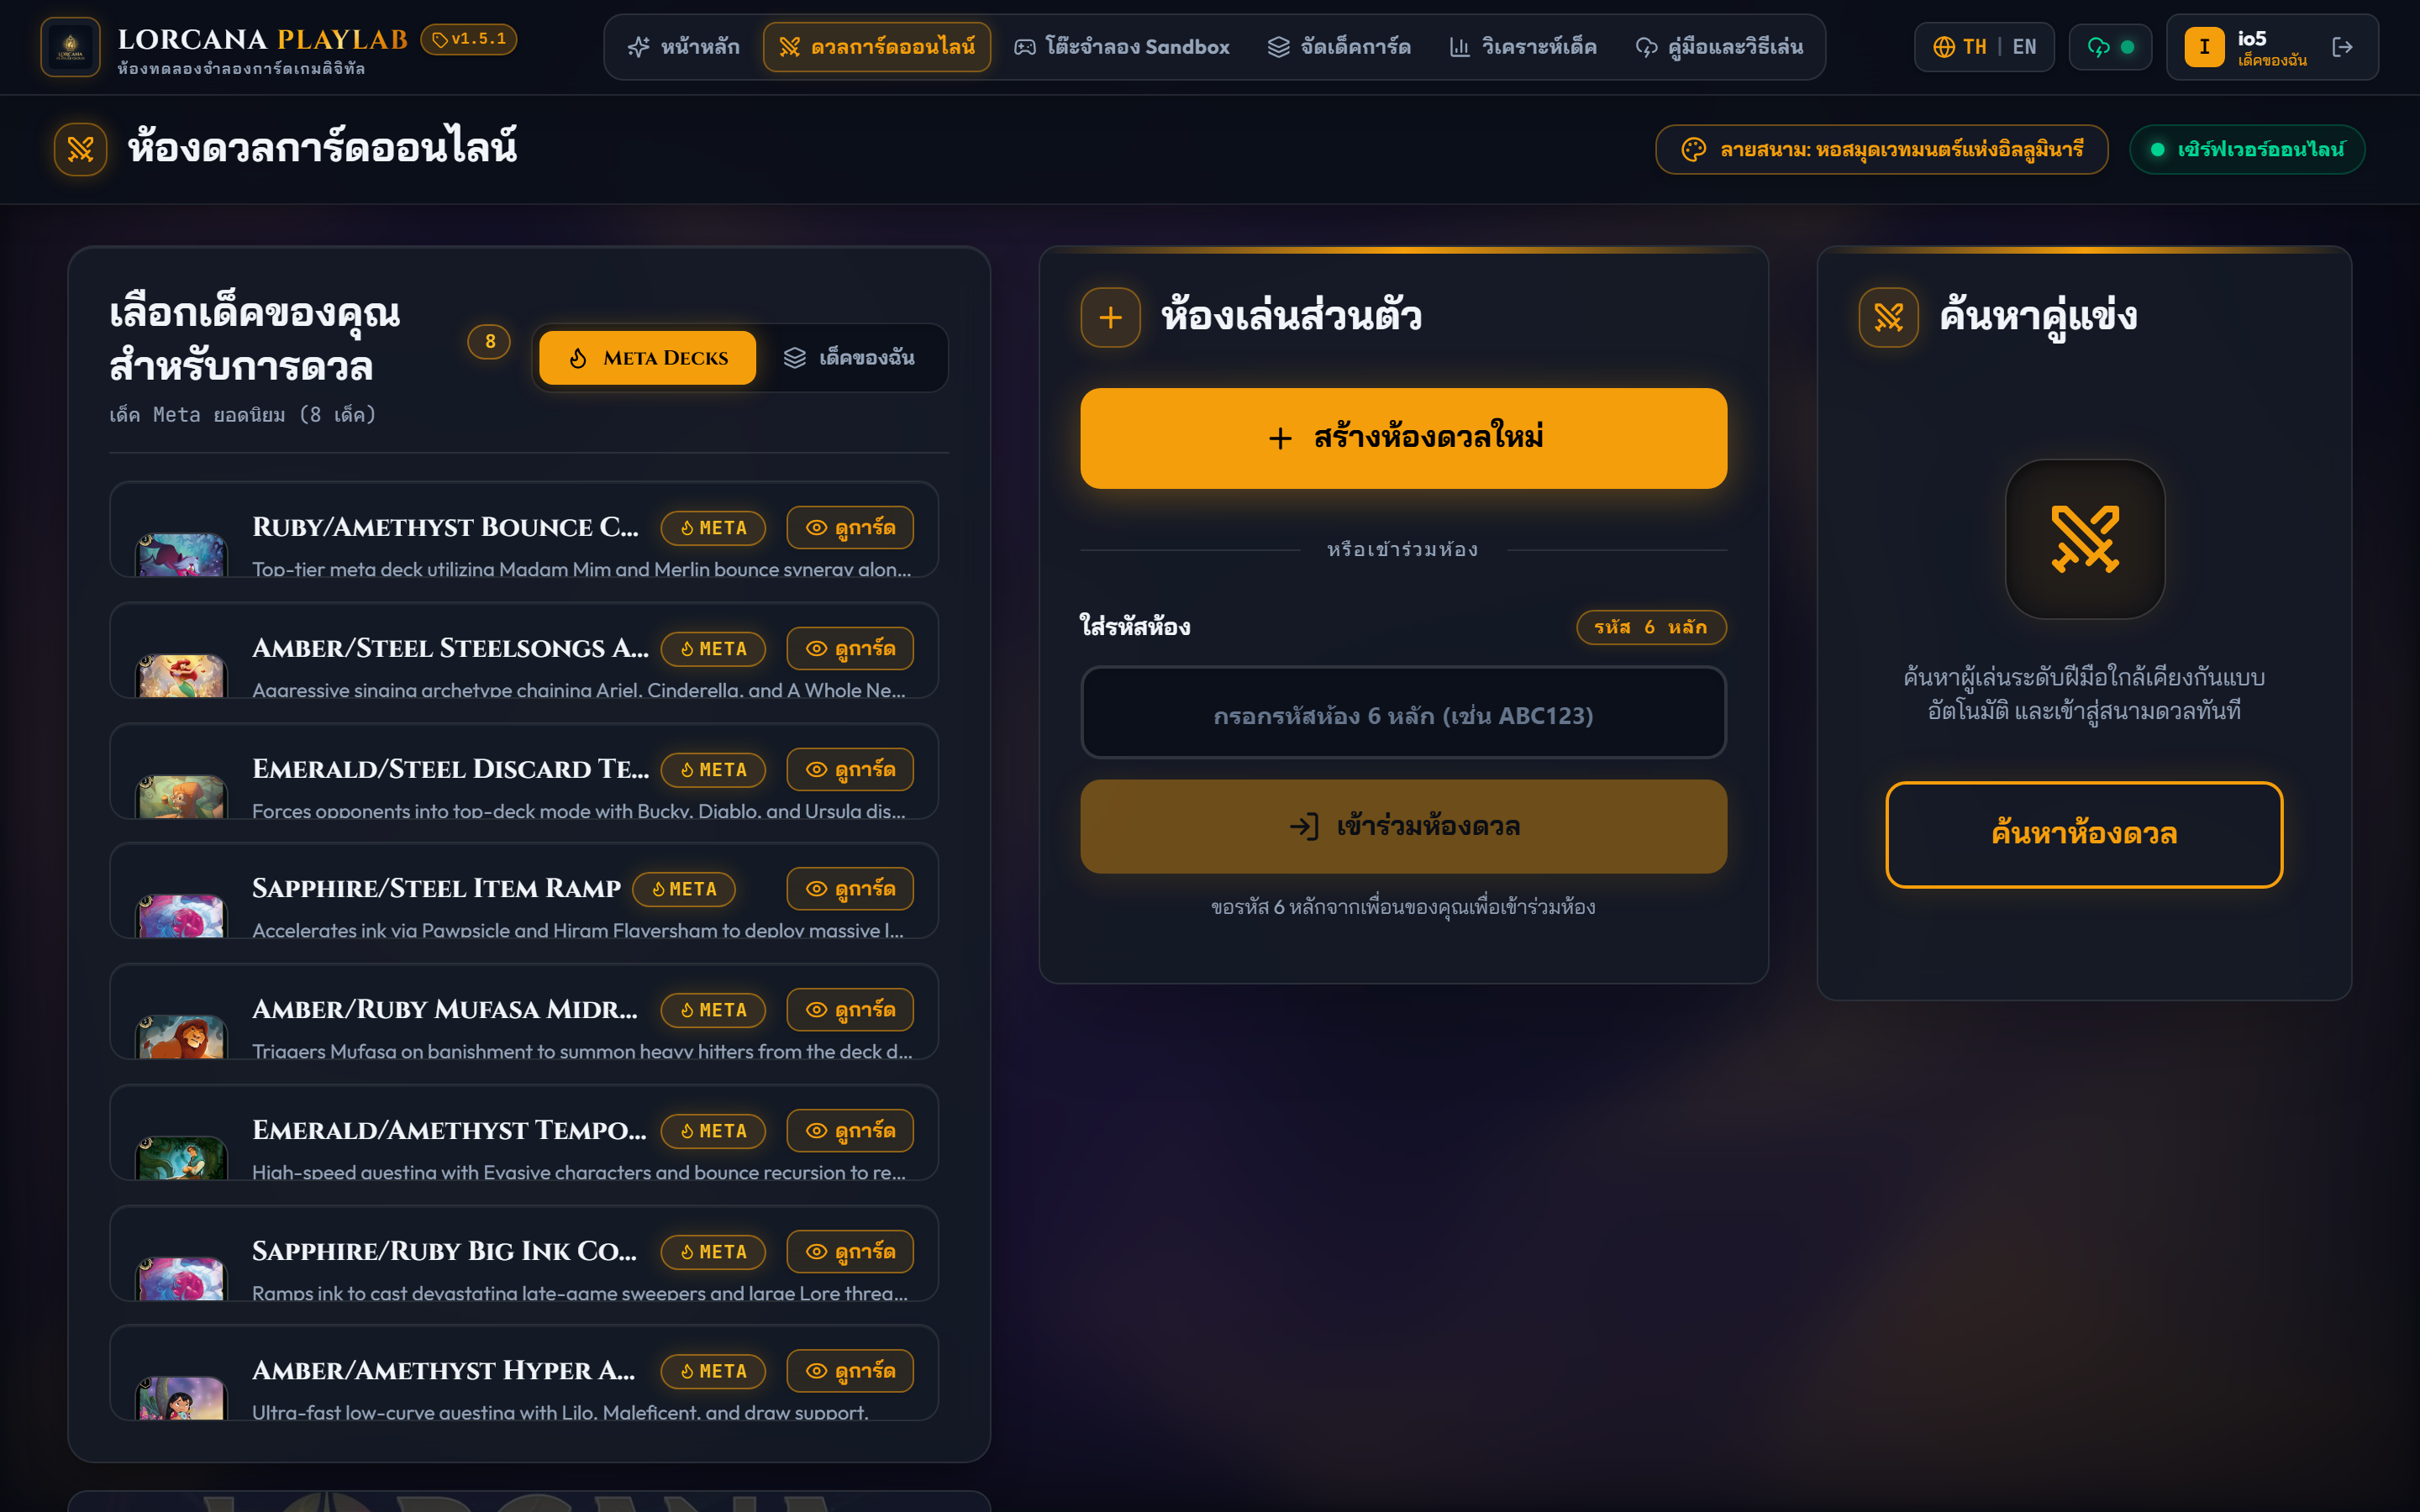
\includegraphics[width=\textwidth]{images/useindoc/05_match_lobby.png}
    \caption{ล็อบบี้สร้างและเข้าห้อง}
\end{subfigure}
\hfill
\begin{subfigure}[b]{0.48\textwidth}
    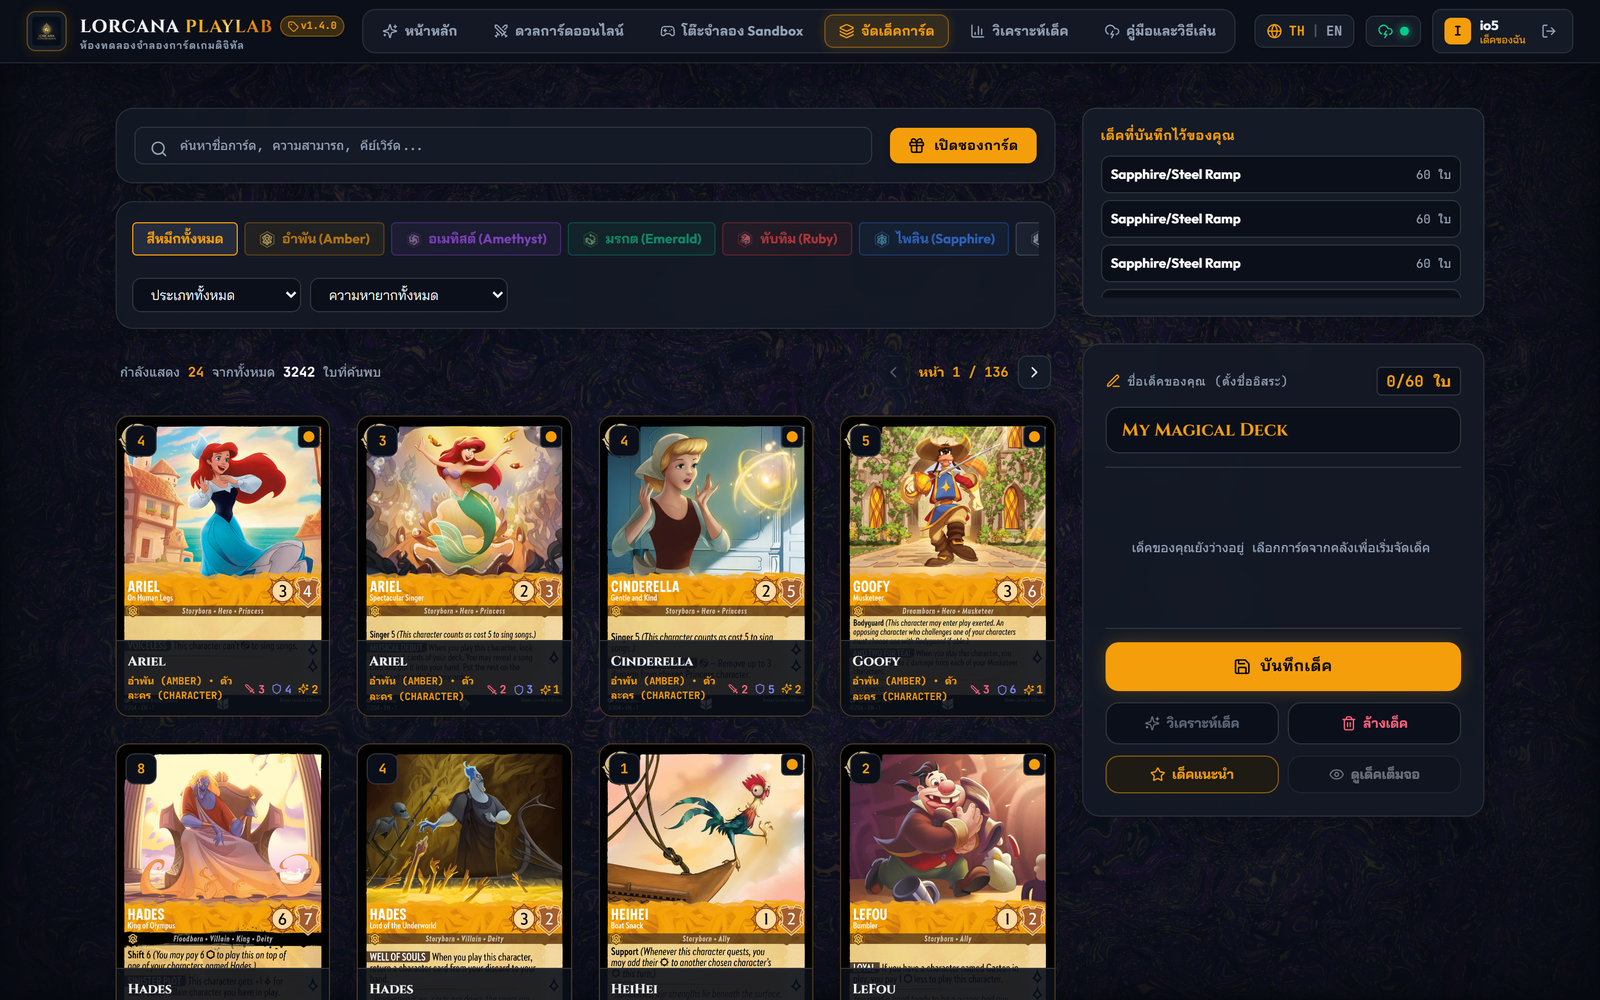
\includegraphics[width=\textwidth]{images/useindoc/04_deck_builder.png}
    \caption{หน้าจัดเด็ค (Deck Builder)}
\end{subfigure}
\\[0.3cm]
\begin{subfigure}[b]{0.48\textwidth}
    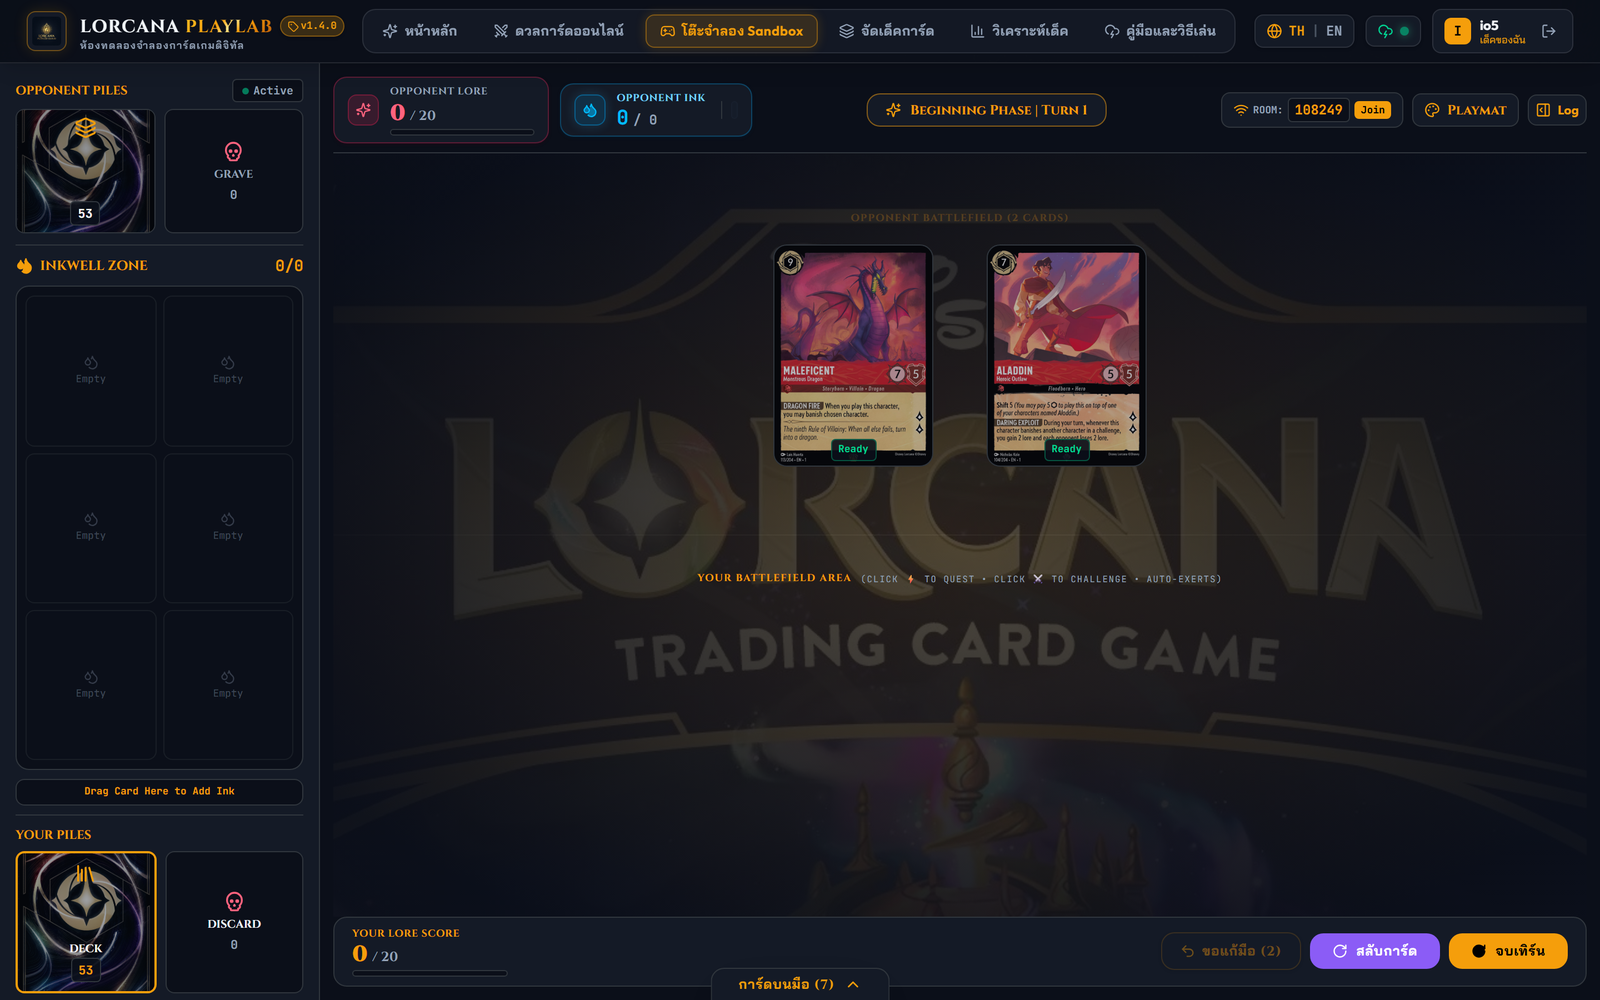
\includegraphics[width=\textwidth]{images/useindoc/07_realtime_room_play.png}
    \caption{กระดานเล่น (Playmat)}
\end{subfigure}
\hfill
\begin{subfigure}[b]{0.48\textwidth}
    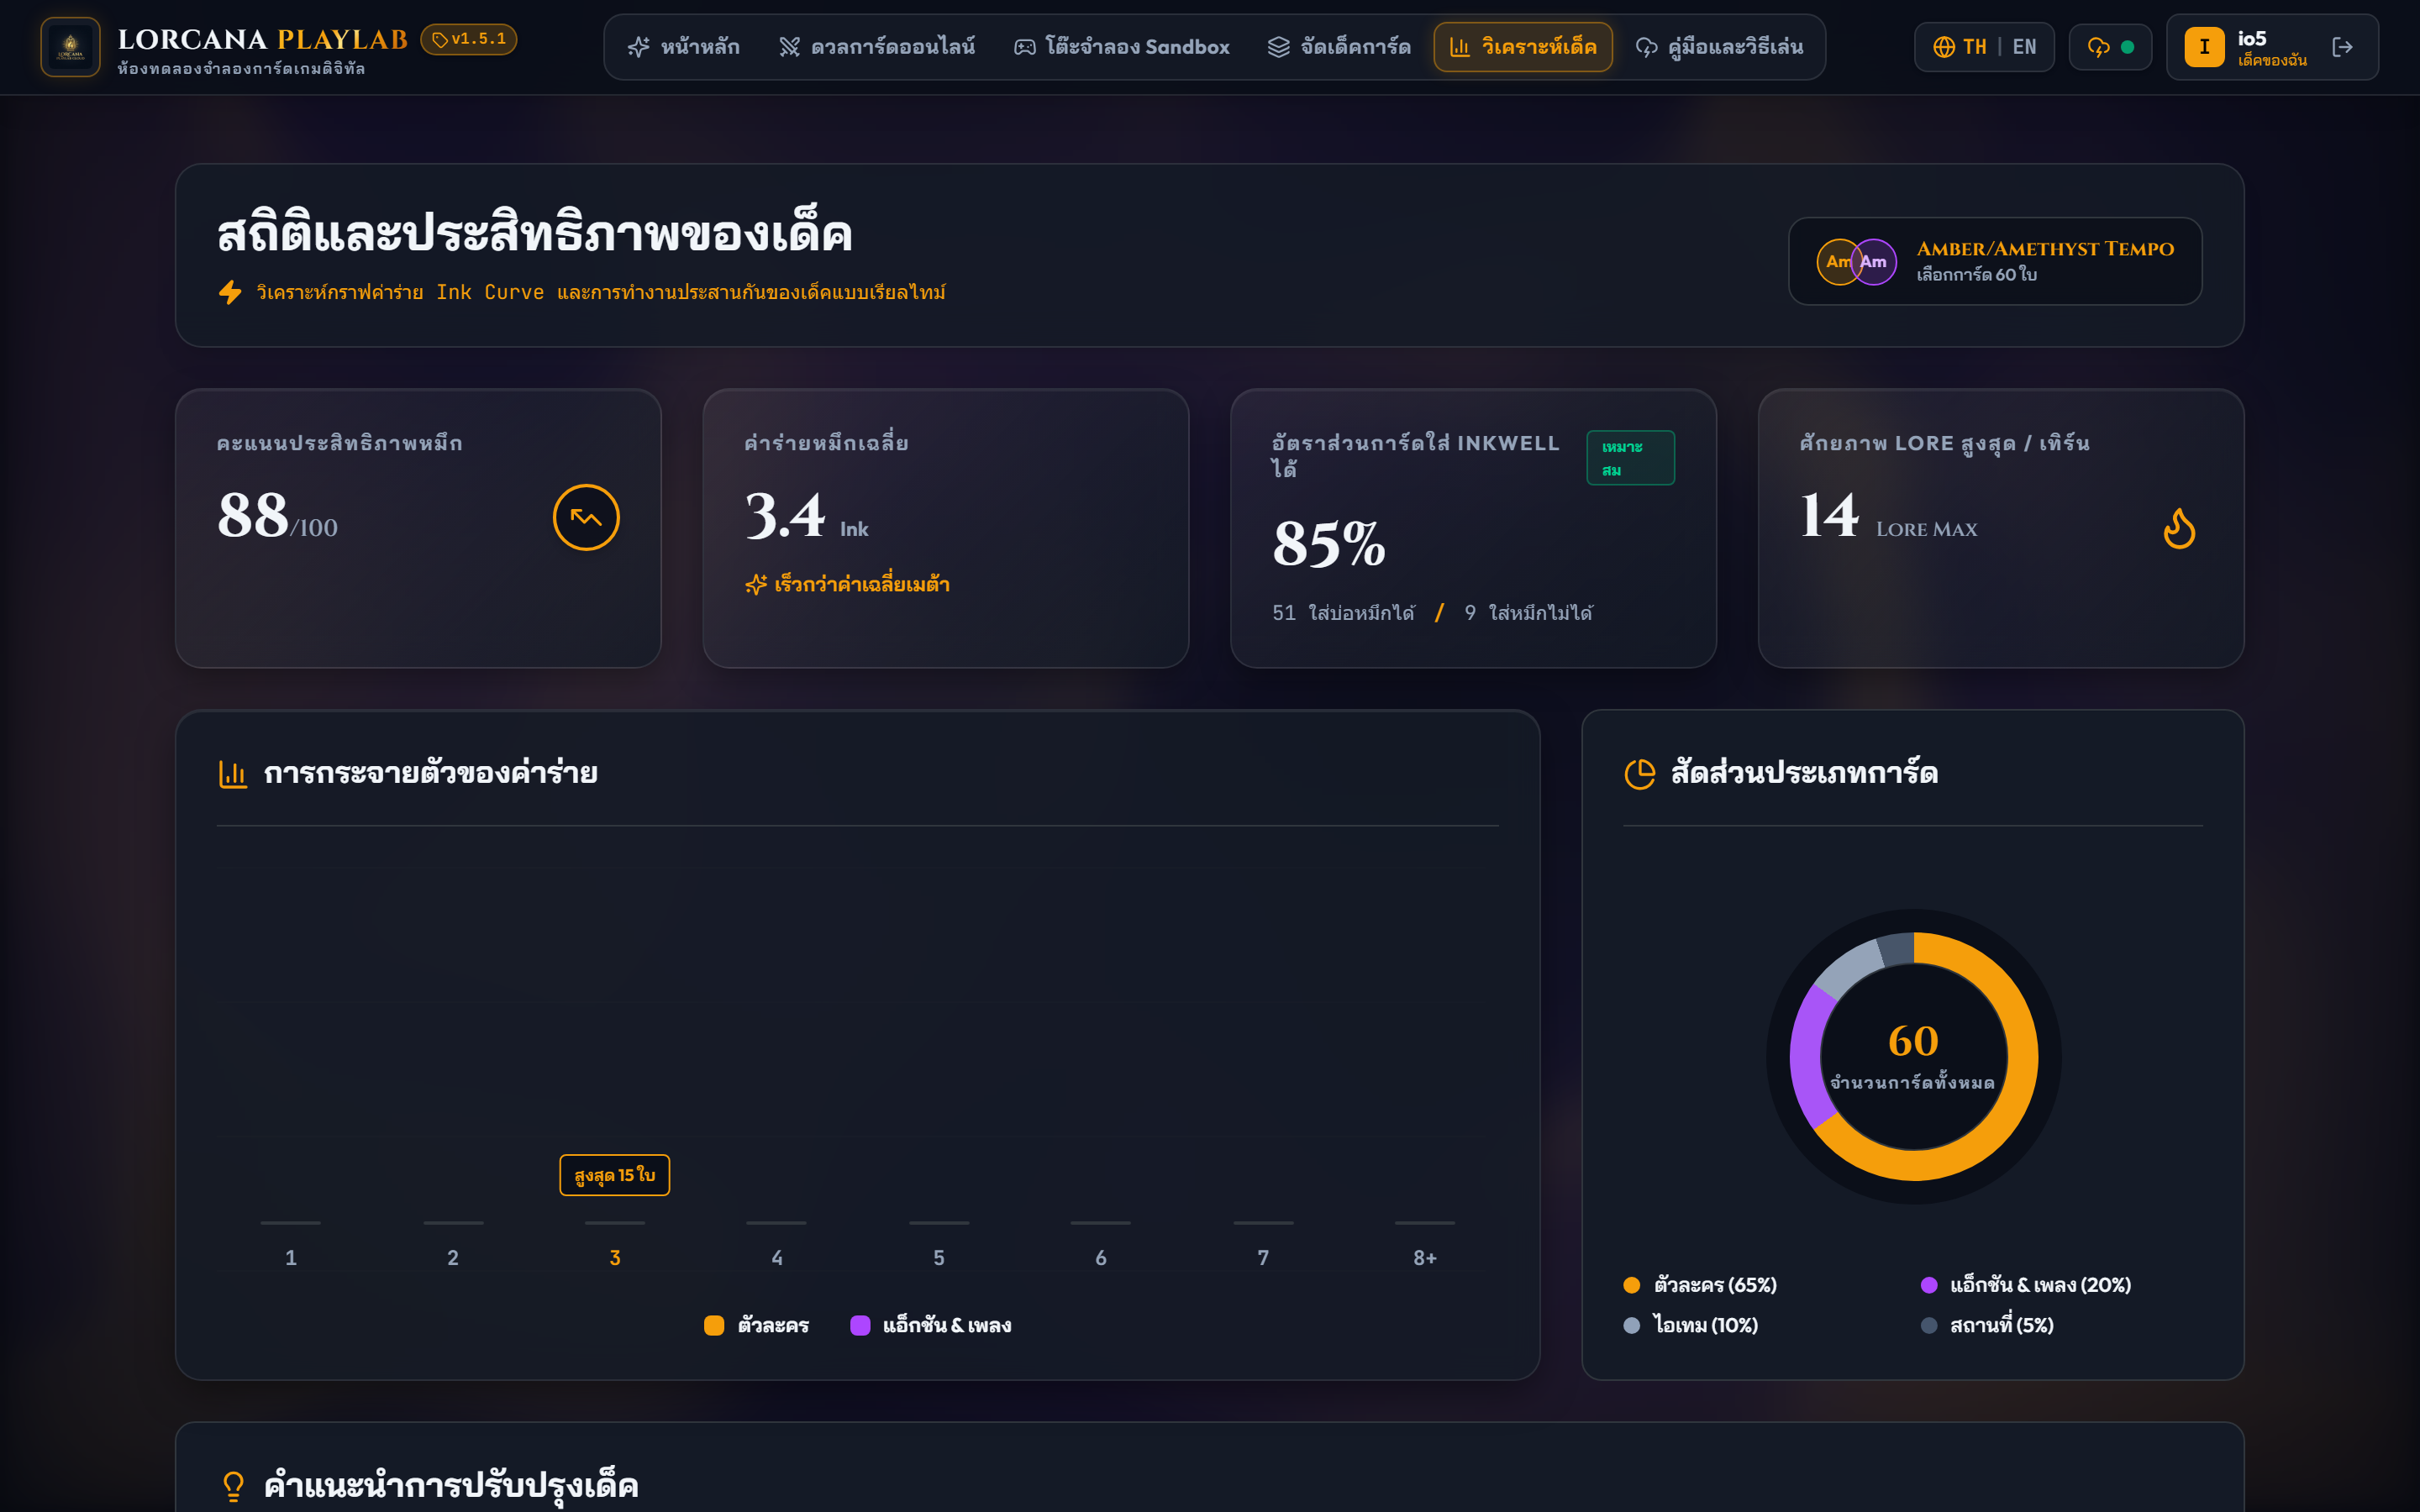
\includegraphics[width=\textwidth]{images/useindoc/09_deck_analytics.png}
    \caption{หน้า Analytics ของเด็ค}
\end{subfigure}
\caption{ภาพหน้าจอของระบบ Disney Lorcana PlayLab Cloud}
\label{fig:ui_showcase}
\end{figure}

องค์ประกอบของกระดานเล่น ได้แก่ พื้นที่สนาม (Play Area) ที่ลากวางการ์ดได้, Inkwell, ตัวนับ Lore 0 ถึง 20, การหมุนการ์ด Ready/Exerted, แถบลำดับเทิร์น (\texttt{TurnPhaseBar}) ที่แสดง \texttt{TURN n}, \texttt{YOUR TURN} และลำดับ Ready, Set, Draw, Main, End (ปุ่มจบเทิร์นอยู่ที่ \texttt{PlayerControlsBar}), หน้าต่าง Dice Duel (\texttt{DiceDuelModal}), หน้าต่าง Mulligan (\texttt{MulliganModal}) และปุ่ม Quest ทุกปุ่มมีป้ายเหตุผลเมื่อทำไม่ได้ เหตุผลมาจากตัวขับเคลื่อนกฎ ไม่ได้เขียนซ้ำใน UI และเล่นครบ 1 เทิร์นได้ด้วยคีย์บอร์ด

ไฟล์ \texttt{LorcanaBoard.tsx} มี 1,617 บรรทัด ณ วันที่ 5 ตุลาคม 2569 \todo{เป้าหมายของ T15 คือต่ำกว่า 1,500 บรรทัด ยังไม่ผ่าน ต้องแยก component เพิ่มก่อนใส่ตัวเลขสุดท้าย}

\section{การทดสอบอัตโนมัติ}

\begin{itemize}
    \item \textbf{Unit และ integration (Vitest 4):} ผ่าน 128 จาก 128 รายการ ใน 20 ไฟล์ (รันเมื่อ 5 ตุลาคม 2569) ครอบคลุมตัวขับเคลื่อนกฎ (TC-ENG), คีย์เวิร์ด (TC-KEY), Ability (TC-AB), Shift/Location/Song/Item (TC-T12), UX (TC-UX), Cache (TC-CACHE) และ Analytics
    \item \textbf{End-to-end (Playwright):} ชุดทดสอบ \texttt{e2e/01} ถึง \texttt{e2e/07} ทำงานกับระบบที่ deploy แล้วเมื่อกำหนด \texttt{E2E\_BASE\_URL} \todo{ใส่จำนวนที่ผ่านทั้งหมดจากการรันรอบสุดท้ายบน stack ที่ deploy ใหม่เมื่อ 5 ตุลาคม 2569}
    \item \textbf{เกมสองผู้เล่น 4 เทิร์น (TC-E2E-25):} เปิด browser สองตัว ทอย Dice Duel เลือก Keep Hand เทิร์น 1 และ 2 ใส่หมึกและลงตัวละคร เทิร์น 3 Quest เทิร์น 4 Challenge ตัวละครที่ Exerted และตรวจว่าหน้าจออีกฝ่ายเห็นการ์ดตรงกัน (\texttt{e2e/07-four-turn-game.spec.ts}) ใช้ 4 เทิร์นเพราะ Challenge เกิดได้เร็วสุดที่เทิร์น 4 (หัวข้อ \ref{sec:challenge}) ชุดทดสอบนี้ไม่ได้ตรวจคีย์เวิร์ดและ Ability เป็นรายใบ เพราะมือเริ่มต้นเป็นการ์ดสุ่ม \textbf{ผล:} ผ่าน 3 จาก 3 รอบติดกันบนระบบที่ deploy เมื่อ 5 ตุลาคม 2569 ใช้เวลา 51.5 ถึง 54.9 วินาทีต่อรอบ (หลักฐาน: \texttt{e2e\_four\_turn\_2026-10-05.txt})
\end{itemize}

ระหว่างสร้างชุดทดสอบ TC-E2E-25 พบข้อบกพร่องในแอป 2 จุด ซึ่งแก้และ deploy ในวันเดียวกัน
\begin{enumerate}
    \item \texttt{TurnPhaseBar} (งาน T13) ผ่าน unit test แต่ไม่เคยถูกแสดงบนกระดานจริง เพราะ \texttt{LorcanaBoard.tsx} import ไว้โดยไม่ได้ใช้ unit test ทดสอบ component เดี่ยวจึงไม่จับข้อนี้ ปัจจุบันแสดงเหนือสนามฝั่งคู่ต่อสู้
    \item ป้ายรายละเอียดการ์ด (quick-glance tooltip) ค้างอยู่หลังการ์ดที่ถูกชี้ออกจากมือ (ลงสนามหรือใส่หมึก) และทับปุ่มจบเทิร์น เพราะการ์ดหายไปก่อนเกิด \texttt{mouseleave} แก้โดยล้างค่าเมื่อการ์ดนั้นไม่อยู่ในมือหรือบนสนามแล้ว
\end{enumerate}
ทั้งสองข้อแสดงว่า unit test ของ component เดี่ยวไม่พอสำหรับยืนยันว่าฟีเจอร์ใช้งานได้ในหน้าจริง ต้องมี end-to-end ที่เล่นผ่านหน้าจอด้วย

\section{การทดลองบน AWS}

การทดลองที่ 1 ถึง 10 ดำเนินการวันที่ 27 และ 29 กันยายน 2569 บน AWS Academy Learner Lab (us-east-1) ไฟล์หลักฐานดิบอยู่ใน \texttt{docs/01\_Reports/stage3\_evidence/}

\subsection{การทดลองที่ 1: เล่นข้ามเครื่อง}

\textbf{คำถาม:} เมื่อมี EC2 2 เครื่อง ผู้เล่นที่ ALB ส่งไปคนละเครื่องเล่นด้วยกันได้หรือไม่

\textbf{วิธี:} Playwright เปิด browser 2 context ผ่าน ALB ผู้เล่น 1 สร้างห้อง ผู้เล่น 2 เข้าด้วยรหัส 6 หลัก ตรวจว่าผู้เล่น 1 เห็นชื่อผู้เล่น 2 ภายใน 10 วินาที

\textbf{ผล:} ผ่าน 5 จาก 5 รอบ ใช้เวลา 9.7 ถึง 14.1 วินาทีต่อรอบ (รวมสมัครสมาชิก เข้าสู่ระบบ และโหลดหน้า) \todo{ไม่มีไฟล์ log ดิบของการทดลองนี้ใน \texttt{stage3\_evidence/} ควรรันซ้ำและเก็บ log}

\subsection{การทดลองที่ 2: ความปลอดภัยบนระบบจริง}

\begin{table}[H]
\centering
\caption{ผลทดสอบความปลอดภัย (OWASP Top 10 [10]: A02, A05, A07)}
\begin{tabularx}{\textwidth}{lX}
\toprule
\textbf{Test Case} & \textbf{ผล} \\
\midrule
TC-AUTH-00a: backend รันโดยไม่มี secret & ก่อนแก้ รันต่อได้ (FAIL) หลังแก้ ออกด้วย exit 1 (PASS) \\
TC-AUTH-00c: รหัส admin ที่เขียนไว้ในโค้ด & ถูกปฏิเสธ (PASS) \\
TC-E2E-16: JWT ที่เซ็นด้วย secret ค่าเริ่มต้น & ได้ 401 ทุกรอบ (10 จาก 10 รอบ) \\
TC-E2E-16: security headers & \texttt{X-Frame-Options: DENY}, \texttt{X-Content-Type-Options: nosniff} \\
Launch template & \texttt{HttpTokens: required} และไม่มี secret ใน user data \\
\bottomrule
\end{tabularx}
\end{table}

\subsection{การทดลองที่ 3: Failover เมื่อ backend ล่ม}

สคริปต์ \texttt{test\_asg\_recovery.ps1} สั่ง \texttt{systemctl stop lorcana-backend} บนเครื่องหนึ่งผ่าน SSM Run Command แล้วจับเวลาจนเครื่องใหม่ healthy และ alarm กลับเป็น OK

\begin{table}[H]
\centering
\caption{ผลการทดลอง Failover (หลักฐาน: \texttt{failover\_app\_*.txt})}
\begin{tabularx}{\textwidth}{lXX}
\toprule
\textbf{เหตุการณ์} & \textbf{รอบ 1 (08:32:50)} & \textbf{รอบ 2 (11:22:57)} \\
\midrule
ASG สั่งเปลี่ยนเครื่อง & T+146 วินาที & T+90 วินาที \\
เครื่องใหม่ healthy & T+231 วินาที & T+166 วินาที \\
Alarm กลับเป็น OK & T+428 วินาที & T+354 วินาที \\
\bottomrule
\end{tabularx}
\end{table}

ALB หยุดส่งทราฟฟิกไปเครื่องที่ล่มภายในราว 30 วินาที (health check 15 วินาที สองครั้ง) ช่วงนั้นคำขออาจได้ 502 เวลากู้คืน 2.8 ถึง 3.9 นาที ส่วนใหญ่เป็นเวลาบูตเครื่องใหม่

\subsection{การทดลองที่ 4: Auto Scaling}

ใช้ \texttt{POST /api/auth/login} (bcrypt cost 10 ใช้ CPU จริง) จาก 40 worker ต่อเนื่อง

\begin{table}[H]
\centering
\caption{ผลการทดลอง Auto Scaling (หลักฐาน: \texttt{stress\_scaling\_*.txt})}
\begin{tabularx}{\textwidth}{lXX}
\toprule
& \textbf{รอบ 1 (process เดียว)} & \textbf{รอบ 2 (cluster 2 worker)} \\
\midrule
CPU เฉลี่ย & 48.7--49.9\% (ค้าง) & 99.8--99.97\% \\
Scale-out & ไม่เกิด & 2 เป็น 4 เครื่อง \\
Login สำเร็จ/ล้มเหลว & ไม่ได้บันทึก & 9,653/0 \\
\bottomrule
\end{tabularx}
\end{table}

\subsection{การทดลองที่ 5: Infrastructure as Code}

\texttt{deploy\_ec2\_vpc\_asg.ps1} สร้าง VPC, subnet 2 AZ, IGW, Security Group, ALB, Target Group, Launch Template, ASG, scaling policy และ alarm สำเร็จ รันซ้ำขณะ stack ยังอยู่จะหยุดด้วย exit 1 ส่วน \texttt{lab.ps1 destroy} ลบทรัพยากรทั้งหมดเหลือแค่ default VPC

เมื่อสร้าง stack ใหม่วันที่ 5 ตุลาคม 2569 พบบั๊กในสคริปต์ \texttt{ensure\_pipeline.ps1}: ตาราง \texttt{LorcanaMatchHistory} และ \texttt{LorcanaPlayerStats} ถูกสร้างด้วยชื่อ key เป็นข้อความ \texttt{\$PkName} ตรงตัว เพราะ PowerShell 7 ไม่แทนค่าตัวแปรในอาร์กิวเมนต์ที่ไม่มีเครื่องหมายคำพูด Lambda ที่ใช้ key \texttt{userId} จึงเขียนตารางไม่ได้ แก้โดยใส่เครื่องหมายคำพูดครอบอาร์กิวเมนต์ แล้วสร้างตารางใหม่ ตรวจ key ได้ \texttt{userId} (และ \texttt{finishedAt\#matchId}) ถูกต้อง

\subsection{การทดลองที่ 6: Content Caching}

\begin{table}[H]
\centering
\caption{ผล Content Caching (หลักฐาน: \texttt{caching\_2026-09-29*.json})}
\begin{tabularx}{\textwidth}{lX}
\toprule
\textbf{ตัวชี้วัด} & \textbf{ค่า} \\
\midrule
ขนาดไฟล์ข้อมูลการ์ดก่อนบีบอัด & 2,351,188 ไบต์ (2.35 MB) \\
ขนาดหลัง gzip & 436,557 ไบต์ (426 KB) ลดลง 81.43\% \\
เวลาโหลดครั้งแรก & 602 มิลลิวินาที \\
เวลาโหลดครั้งที่สอง (cache hit) & 86 มิลลิวินาที \\
ข้อมูลรับส่งครั้งที่สอง & 0 ไบต์ (ใช้แคชในเบราว์เซอร์) \\
\bottomrule
\end{tabularx}
\end{table}

\subsection{การทดลองที่ 7: Dead Letter Queue}

ข้อความ JSON เสียหายถูกส่งเข้าคิววิเคราะห์เด็ค Lambda ส่งคืน \texttt{batchItemFailures} ข้อความถูกลองซ้ำครบ 3 ครั้ง (\texttt{maxReceiveCount: 3}) แล้วเข้า DLQ ที่ T+102 วินาที จำนวนข้อความค้างในคิวหลัก 0 ข้อความ (หลักฐาน: \texttt{dlq\_20260929\_131824.log})

\subsection{การทดลองที่ 8: SNS Fan-out}

เทสต์ TC-E2E-23 (สมัคร เข้าสู่ระบบ สร้างเด็ค จบเกม แล้วรอจนผลปรากฏในประวัติและสถิติของทั้งสองผู้เล่น) ใช้เวลารวม 4.9 วินาที จึงสรุปได้ว่าการกระจายผลใช้เวลาไม่เกิน 5 วินาทีหลังจบเกม (ยังไม่ได้แยกวัดเฉพาะช่วง SNS ถึง DynamoDB) การป้องกันการเข้าถึง (OWASP A01): ส่งผลโดยไม่มี JWT ได้ 401 ส่งผลของแมตช์ที่ตนไม่ได้เล่นได้ 403 (หลักฐาน: \texttt{decoupling\_match\_events\_20260929.log})

\subsection{การทดลองที่ 9: ElastiCache แบบ Cache-Aside}

\textbf{วิธี:} \texttt{measure\_leaderboard.mjs} เรียก \texttt{GET /api/leaderboard} ผ่าน ALB 8 รอบ แต่ละรอบรอให้ TTL 60 วินาทีหมดก่อน 1 คำขอ (ควรได้ MISS) แล้วยิงต่อเนื่อง 13 คำขอ (ควรได้ HIT) แยกกลุ่มตาม header \texttt{X-Cache} ที่ server ตอบ ค่า \texttt{durationMs} วัดภายใน backend ส่วนค่าฝั่ง client รวมความหน่วงเครือข่ายด้วย

\begin{table}[H]
\centering
\caption{ผลตารางผู้นำ (ค่ามัธยฐานและ p95 หลักฐาน: \nolinkurl{leaderboard_cache_2026-09-29T17-18-08-612Z.json})}
\begin{tabularx}{\textwidth}{Xrrr}
\toprule
\textbf{สถานการณ์} & \textbf{ตัวอย่าง} & \textbf{server (p95)} & \textbf{client (p95)} \\
\midrule
Cache Miss (อ่าน DynamoDB) & 8 & 41 ms (112) & 562.7 ms (814.2) \\
Cache Hit (ภายใน TTL 60 วินาที) & 104 & 1 ms (2) & 247.5 ms (255.9) \\
\bottomrule
\end{tabularx}
\end{table}

เวลาฝั่ง server ลดจาก 41 เหลือ 1 มิลลิวินาที (ลดลง 97.56\%) เวลาที่ผู้ใช้เห็นลดจาก 562.7 เหลือ 247.5 มิลลิวินาที เพราะความหน่วงเครือข่ายราว 247 มิลลิวินาทีแคชลดไม่ได้ กลุ่ม MISS มีเพียง 8 ตัวอย่างเพราะต้องรอ TTL 62 วินาทีต่อ 1 ตัวอย่าง และตารางสถิติมีข้อมูลน้อย ค่า MISS บนตารางใหญ่กว่านี้จะสูงขึ้น เมื่อแคชขัดข้องระบบอ่าน DynamoDB โดยตรงและตอบ HTTP 200 (ทดสอบด้วย unit test TC-LEAD-04 และ TC-CACHE-004)

\textbf{ปัญหาที่พบ:} รอบแรกได้ MISS ตลอด สาเหตุคือ Redis client เชื่อมต่อตอนมีคำขอแรกและตั้ง \texttt{enableOfflineQueue: false} คำขอแรกของทุก process จึงล้มเงียบแล้วไปอ่าน DynamoDB แก้โดยเชื่อมต่อตอน server เริ่ม (\texttt{warmCache()}) และเพิ่ม unit test TC-CACHE-001 ถึง 004 หลังแก้ TC-E2E-24 ได้ MISS แล้ว HIT ตามที่ออกแบบ

\subsection{การทดลองที่ 10: Ability Coverage}

\texttt{measure\_ability\_coverage.ts} วิเคราะห์การ์ด 3,242 ใบ (Set 1 ถึง 13) พบ Ability 3,768 ข้อ (หลักฐาน: \texttt{ability\_coverage.json})

\begin{table}[H]
\centering
\caption{ระดับการรองรับ Ability ของตัวขับเคลื่อนกฎ}
\begin{tabularx}{\textwidth}{lrX}
\toprule
\textbf{ระดับ} & \textbf{จำนวน (\%)} & \textbf{คำอธิบาย} \\
\midrule
Full Support & 609 (16.16\%) & ระบบคำนวณและเลือกเป้าหมายอัตโนมัติ \\
Partial Support & 203 (5.39\%) & ตรวจจังหวะ trigger ได้ ต้องระบุเพิ่มเติม \\
Manual Resolve & 2,956 (78.45\%) & แสดงป้ายให้ผู้เล่นจัดการเอง \\
\bottomrule
\end{tabularx}
\end{table}

\subsection{ภาพหลักฐานจาก AWS Console}

ภาพในหัวข้อนี้แคปจาก AWS Console ภูมิภาค us-east-1 เมื่อวันที่ 12 ตุลาคม 2569 หลังสร้าง stack ใหม่และ publish โค้ดล่าสุด ภาพอยู่ใน \texttt{docs/01\_Reports/images/useindoc/} ไฟล์ขึ้นต้นด้วย \texttt{aws\_2026-10-12\_}

\begin{figure}[H]
\centering
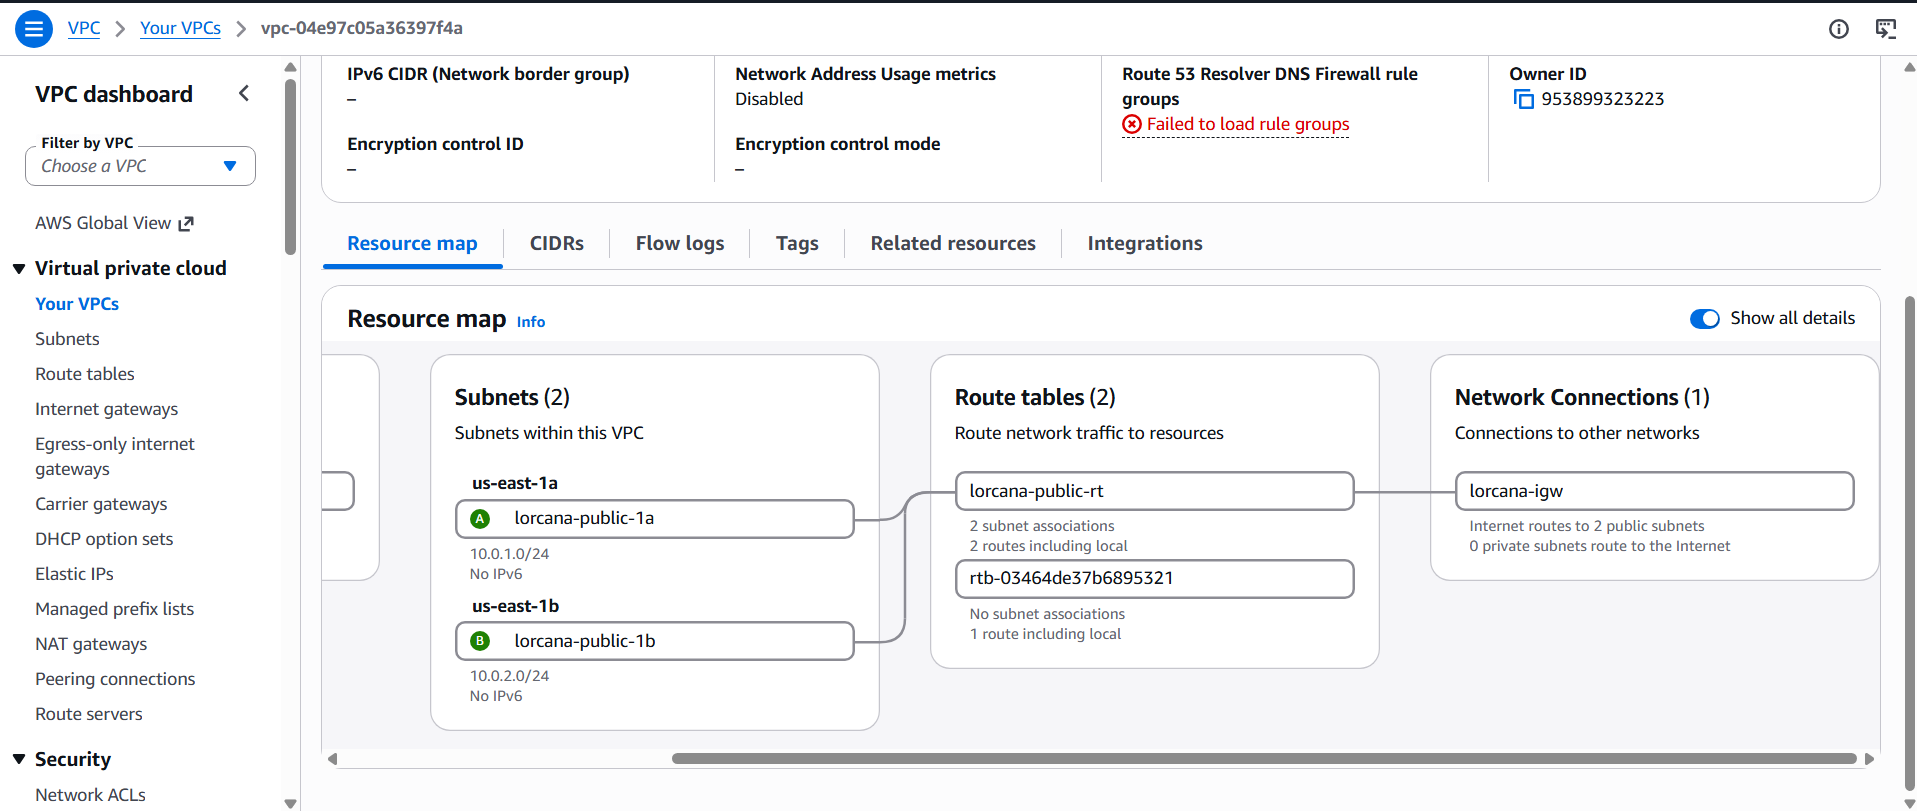
\includegraphics[width=\textwidth]{images/useindoc/aws_2026-10-12_vpc_resource_map.png}
\caption{Resource map ของ VPC \texttt{lorcana-lean-vpc} (10.0.0.0/16): subnet สาธารณะ \texttt{lorcana-public-1a} และ \texttt{lorcana-public-1b} ใน 2 Availability Zone, route table \texttt{lorcana-public-rt} ผูกกับทั้งสอง subnet และเชื่อม \texttt{lorcana-igw} ไม่มี private subnet และไม่มี NAT Gateway}
\label{fig:aws_vpc_map}
\end{figure}

\begin{figure}[H]
\centering
\begin{subfigure}[b]{0.48\textwidth}
    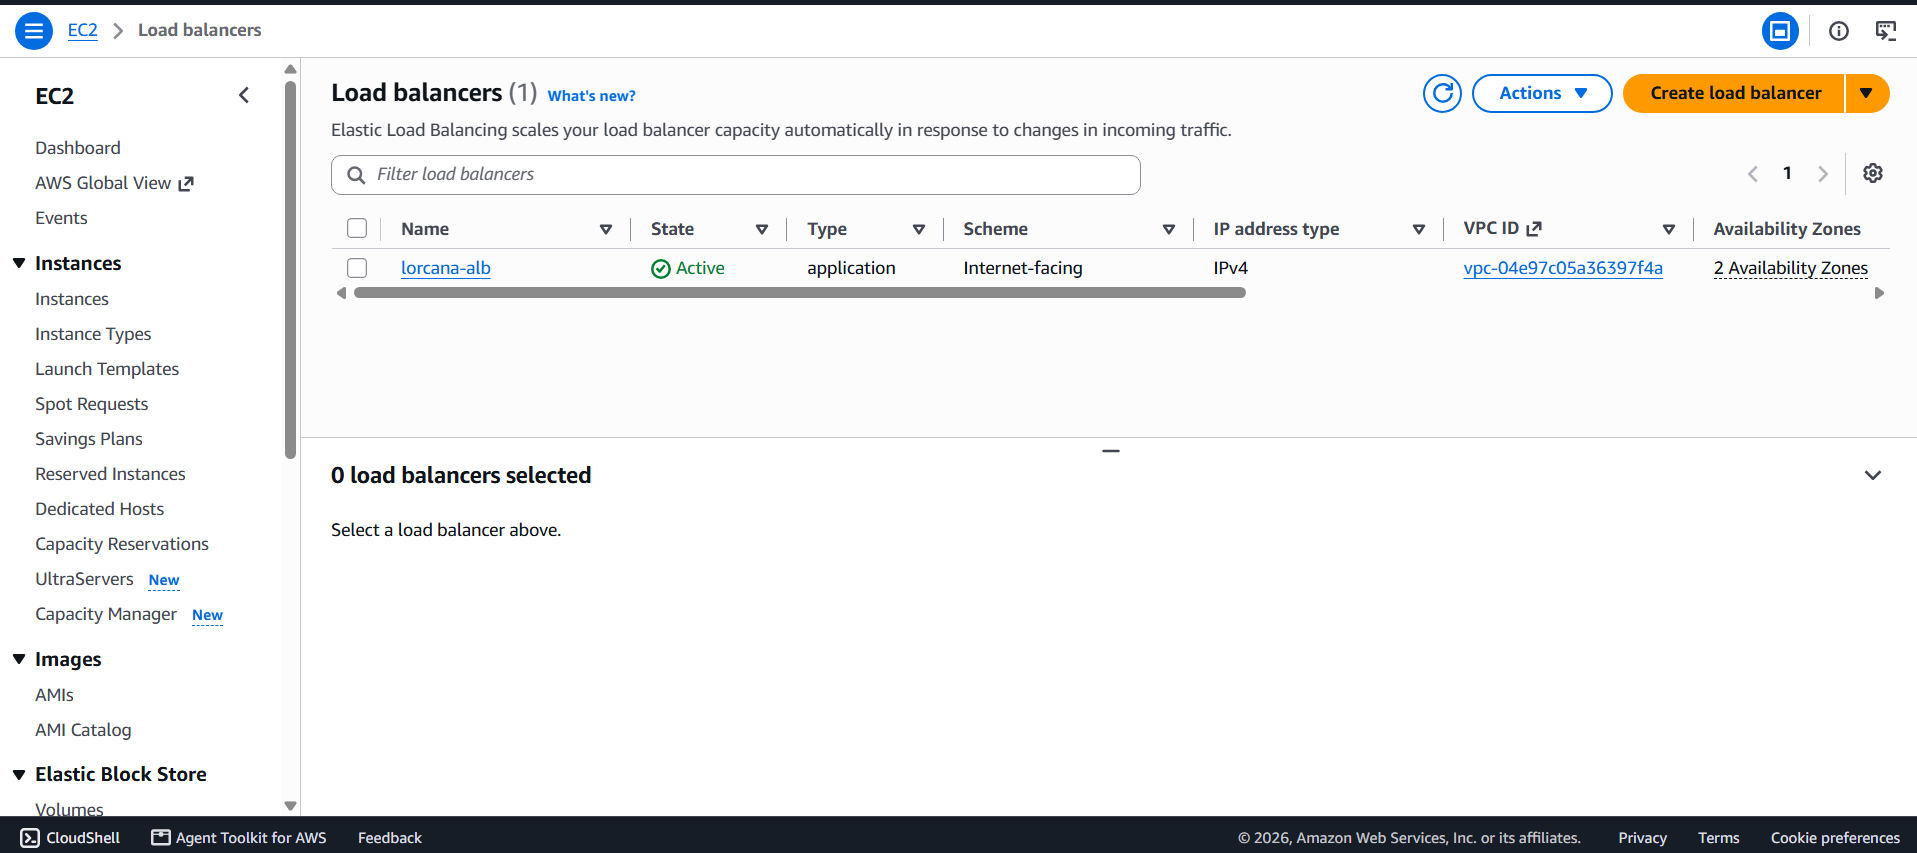
\includegraphics[width=\textwidth]{images/useindoc/aws_2026-10-12_alb_active.png}
    \caption{\texttt{lorcana-alb} สถานะ Active, Internet-facing, 2 Availability Zone}
\end{subfigure}
\hfill
\begin{subfigure}[b]{0.48\textwidth}
    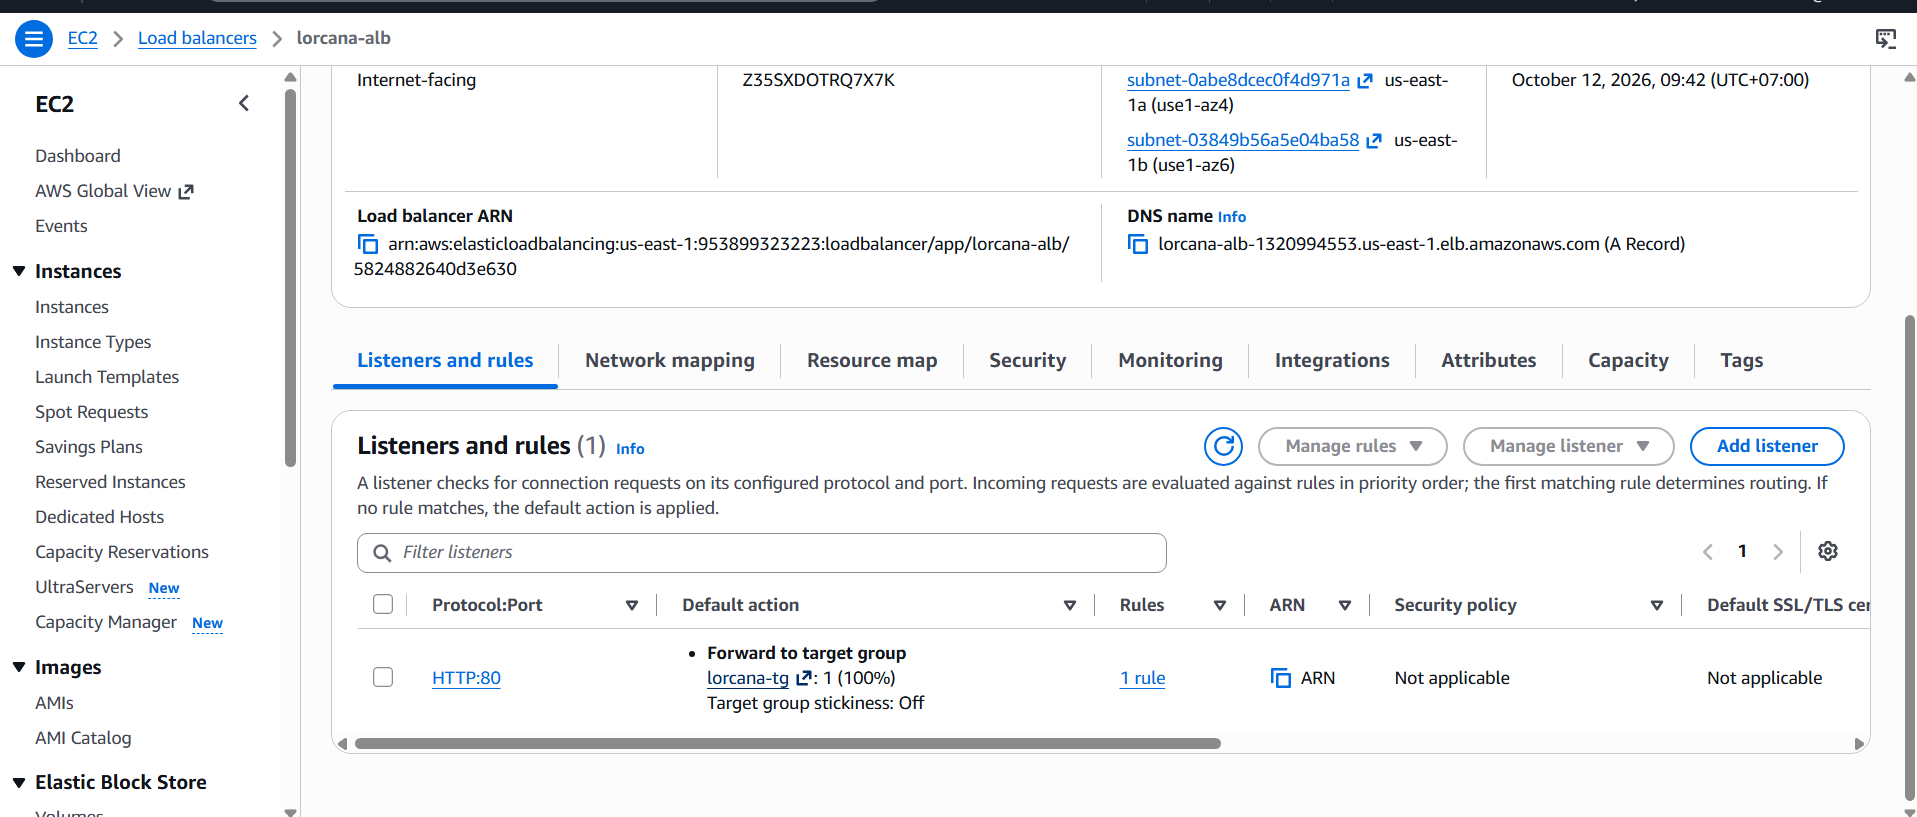
\includegraphics[width=\textwidth]{images/useindoc/aws_2026-10-12_alb_listener.png}
    \caption{Listener HTTP:80 ส่งต่อไปยัง target group \texttt{lorcana-tg}}
\end{subfigure}
\caption{Application Load Balancer ของระบบ}
\label{fig:aws_alb}
\end{figure}

\begin{figure}[H]
\centering
\begin{subfigure}[b]{0.48\textwidth}
    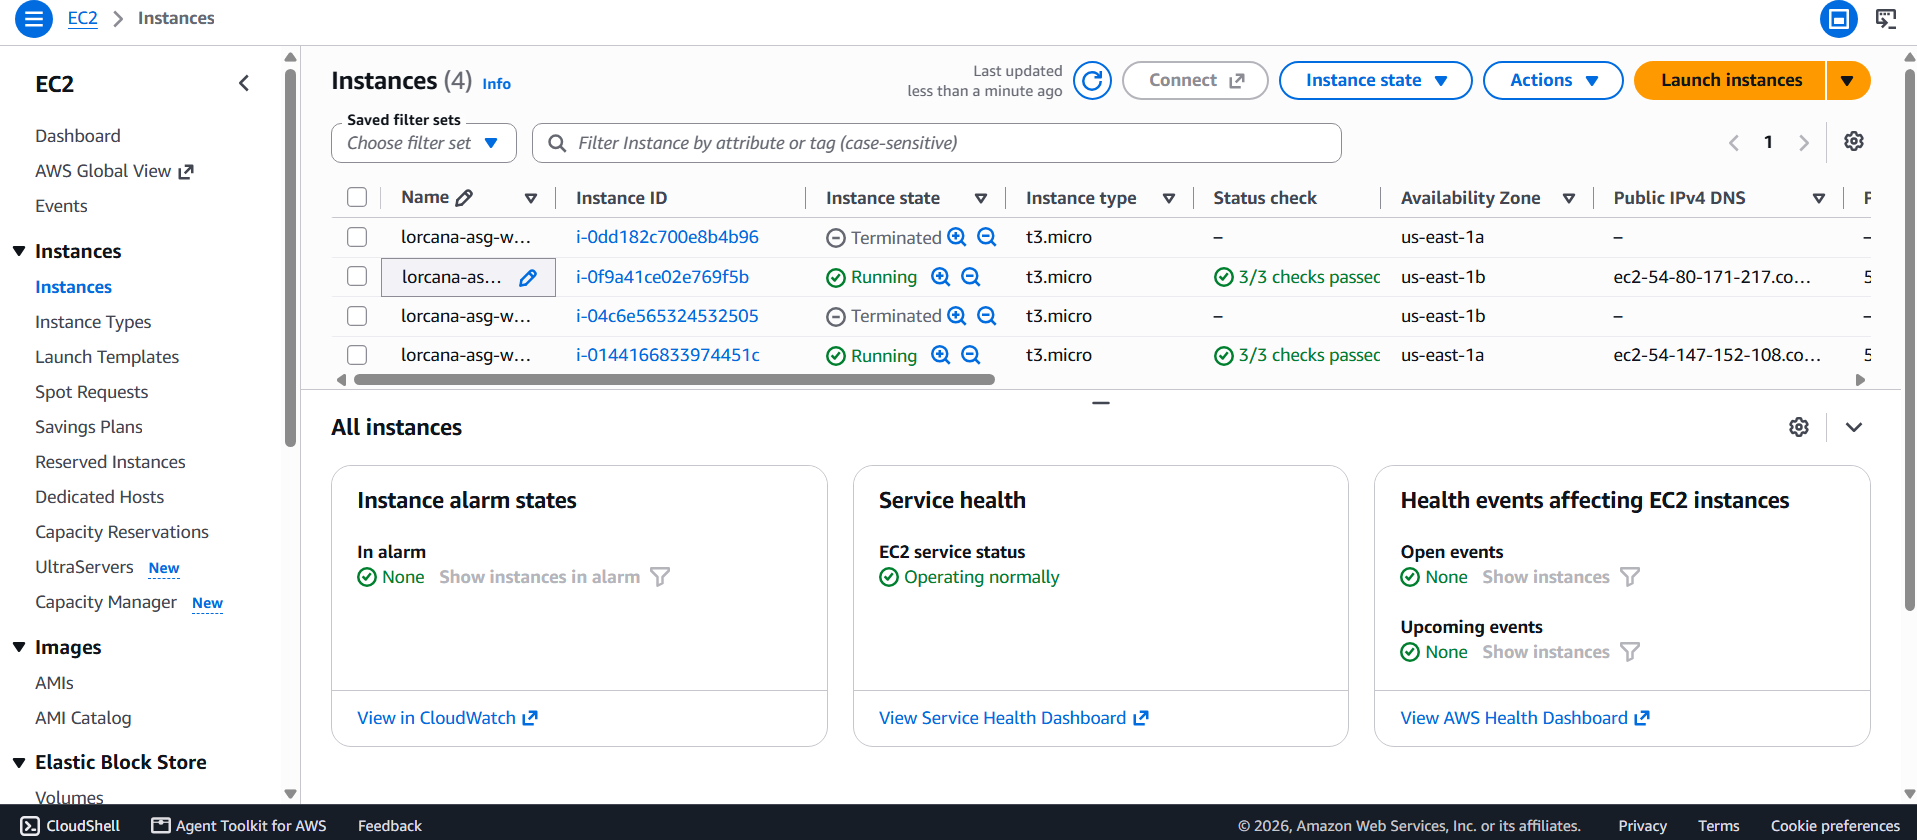
\includegraphics[width=\textwidth]{images/useindoc/aws_2026-10-12_ec2_instances.png}
    \caption{EC2 ที่กำลังทำงาน 2 เครื่อง ใน \texttt{us-east-1a} และ \texttt{us-east-1b} ผ่าน status check 3/3 ส่วนอีก 2 เครื่องเป็นเครื่องเก่าที่ถูกแทนที่ (Terminated)}
\end{subfigure}
\hfill
\begin{subfigure}[b]{0.48\textwidth}
    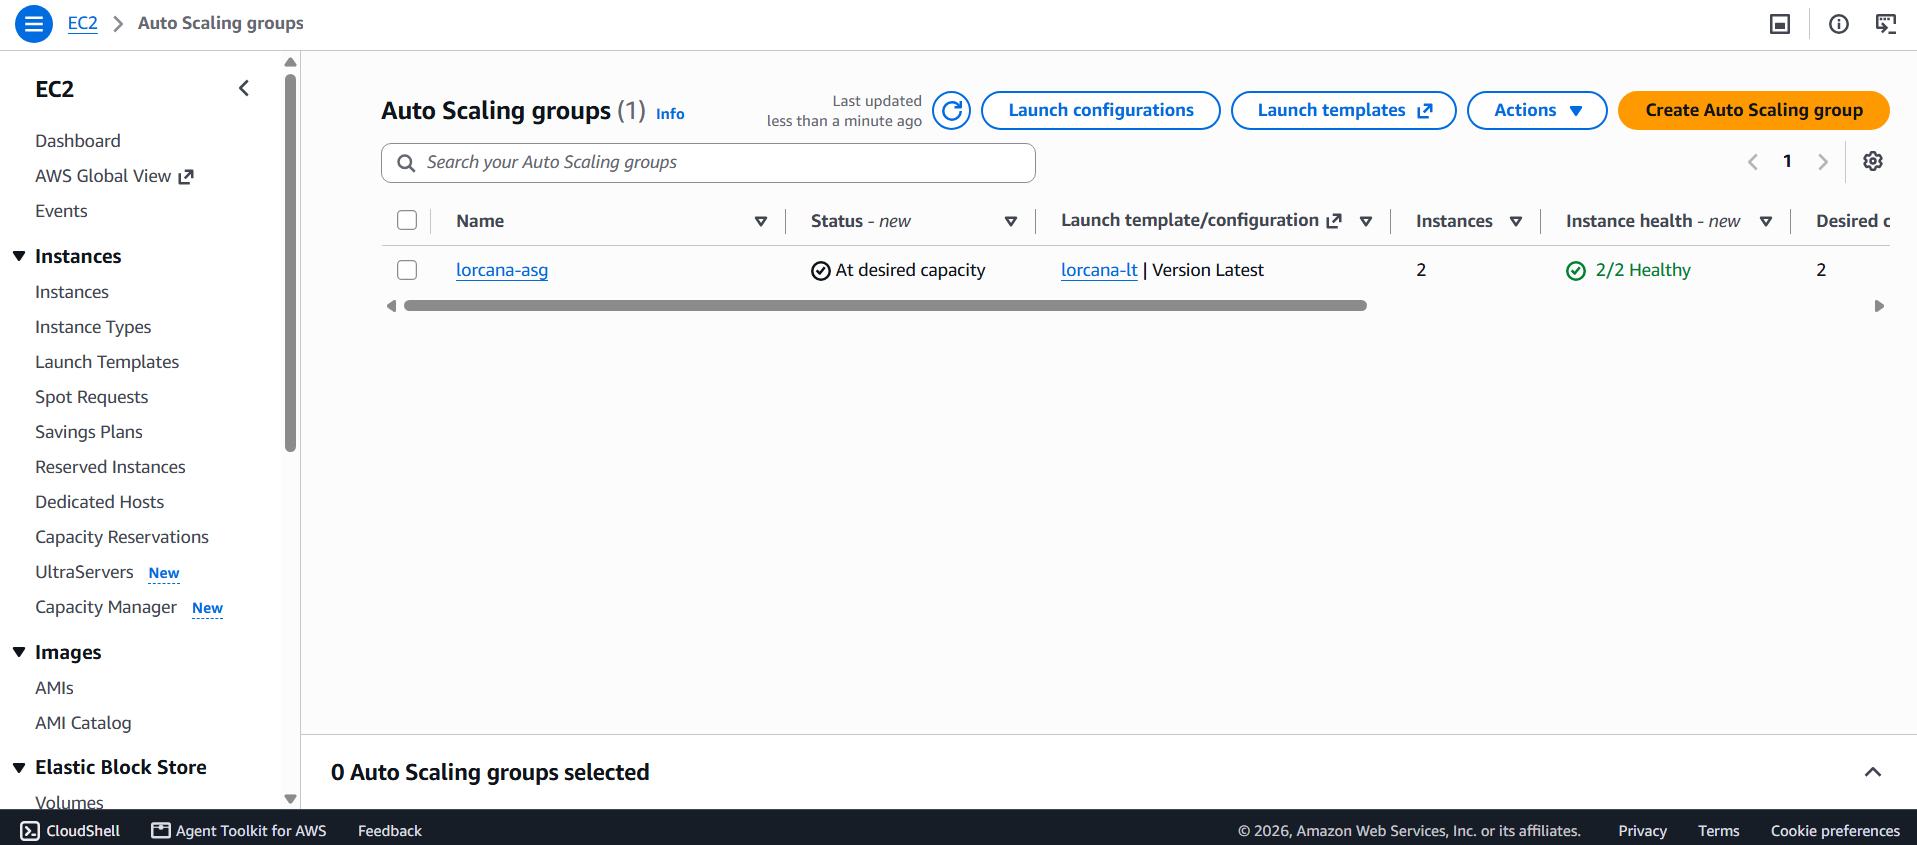
\includegraphics[width=\textwidth]{images/useindoc/aws_2026-10-12_asg_overview.png}
    \caption{Auto Scaling group \texttt{lorcana-asg} At desired capacity, 2 เครื่อง สถานะ 2/2 Healthy}
\end{subfigure}
\caption{เครื่อง EC2 และ Auto Scaling group}
\label{fig:aws_ec2_asg}
\end{figure}

\begin{figure}[H]
\centering
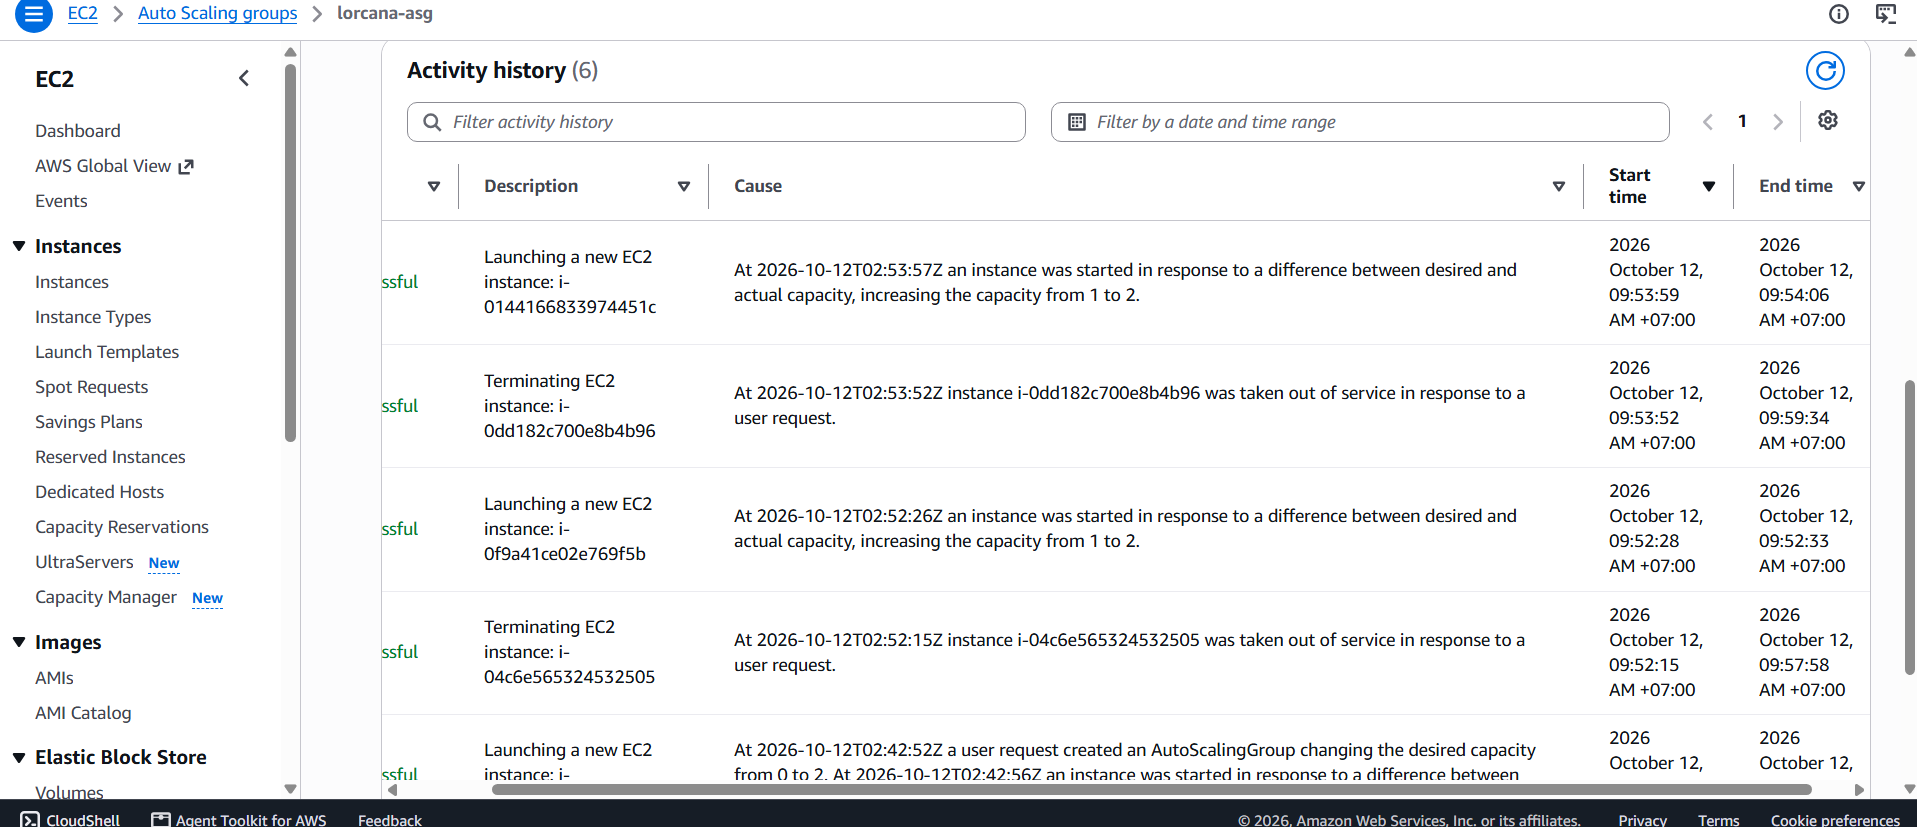
\includegraphics[width=\textwidth]{images/useindoc/aws_2026-10-12_asg_activity.png}
\caption{Activity history ของ \texttt{lorcana-asg}: การเปลี่ยนเครื่องทีละเครื่อง (terminate เครื่องเก่า แล้ว launch เครื่องใหม่ทดแทน) ระหว่าง \texttt{lab.ps1 publish} และการเพิ่มจำนวนเครื่องจาก 0 เป็น 2 เมื่อสร้าง stack}
\label{fig:aws_asg_activity}
\end{figure}

\begin{figure}[H]
\centering
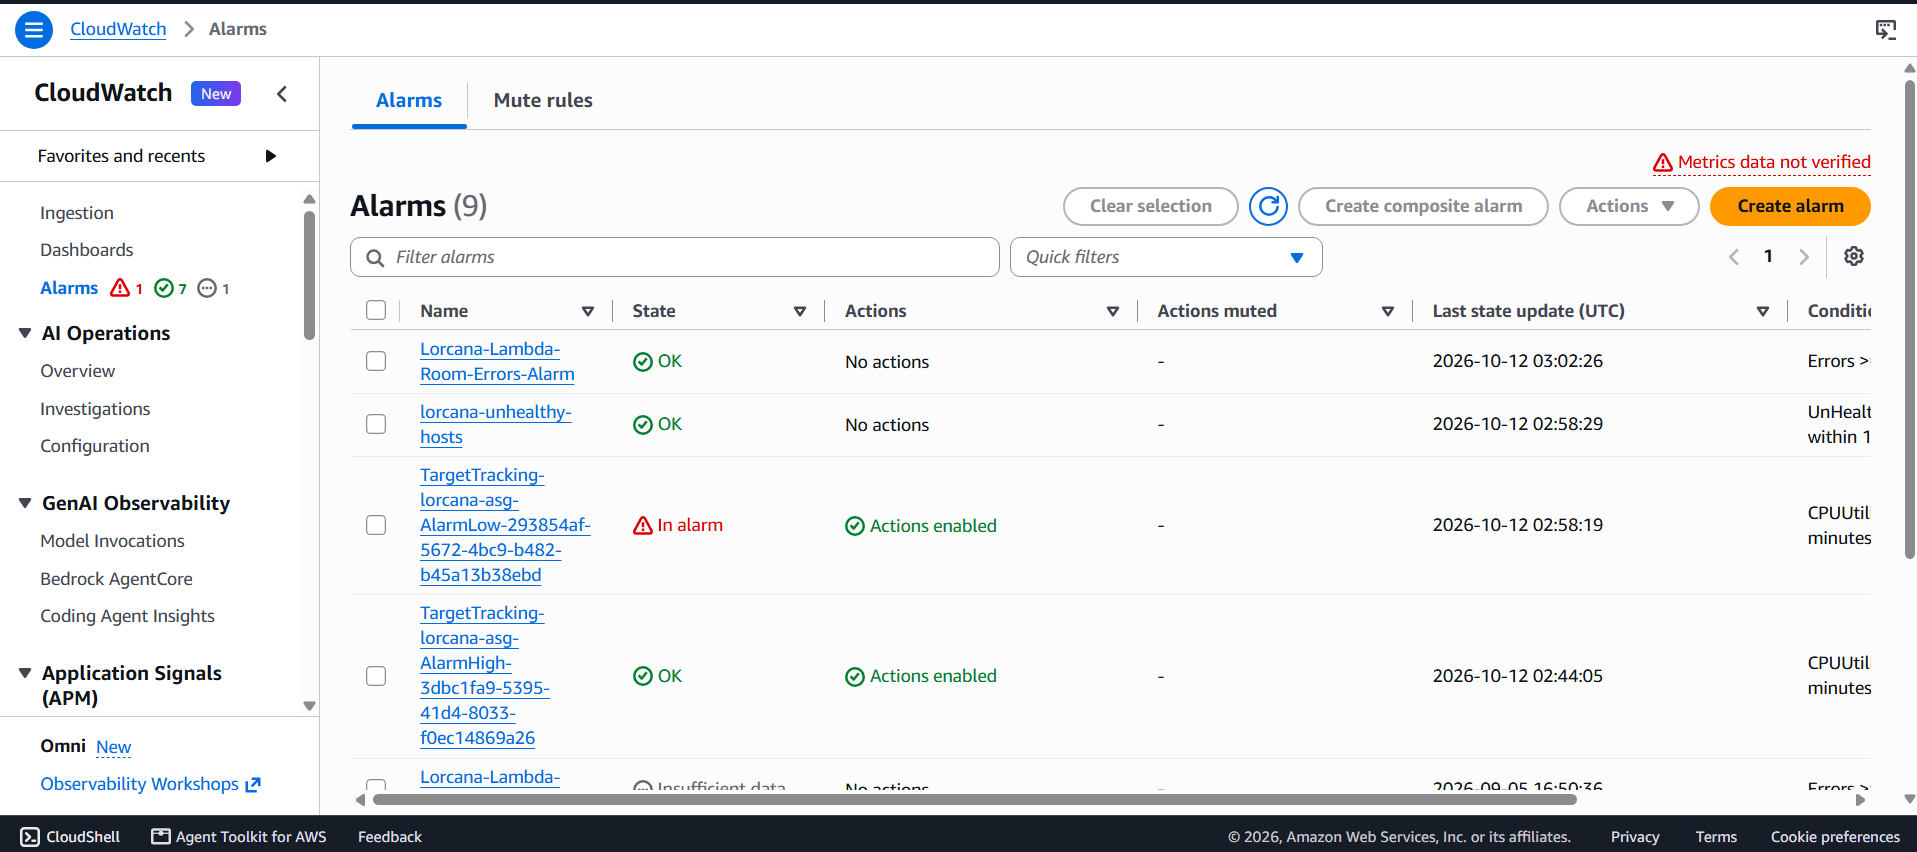
\includegraphics[width=\textwidth]{images/useindoc/aws_2026-10-12_cloudwatch_alarms.png}
\caption{CloudWatch Alarms: \texttt{lorcana-unhealthy-hosts} และ alarm ของ target tracking \texttt{AlarmHigh} อยู่สถานะ OK ส่วน \texttt{AlarmLow} อยู่สถานะ In alarm ตามปกติเมื่อโหลดต่ำ (CPU ต่ำกว่าเป้า) ระบบไม่ลดจำนวนเครื่องเพราะ MinSize เท่ากับ 2 ภาพนี้ไม่ใช่หลักฐานการเพิ่มเครื่อง}
\label{fig:aws_cloudwatch}
\end{figure}

\begin{figure}[H]
\centering
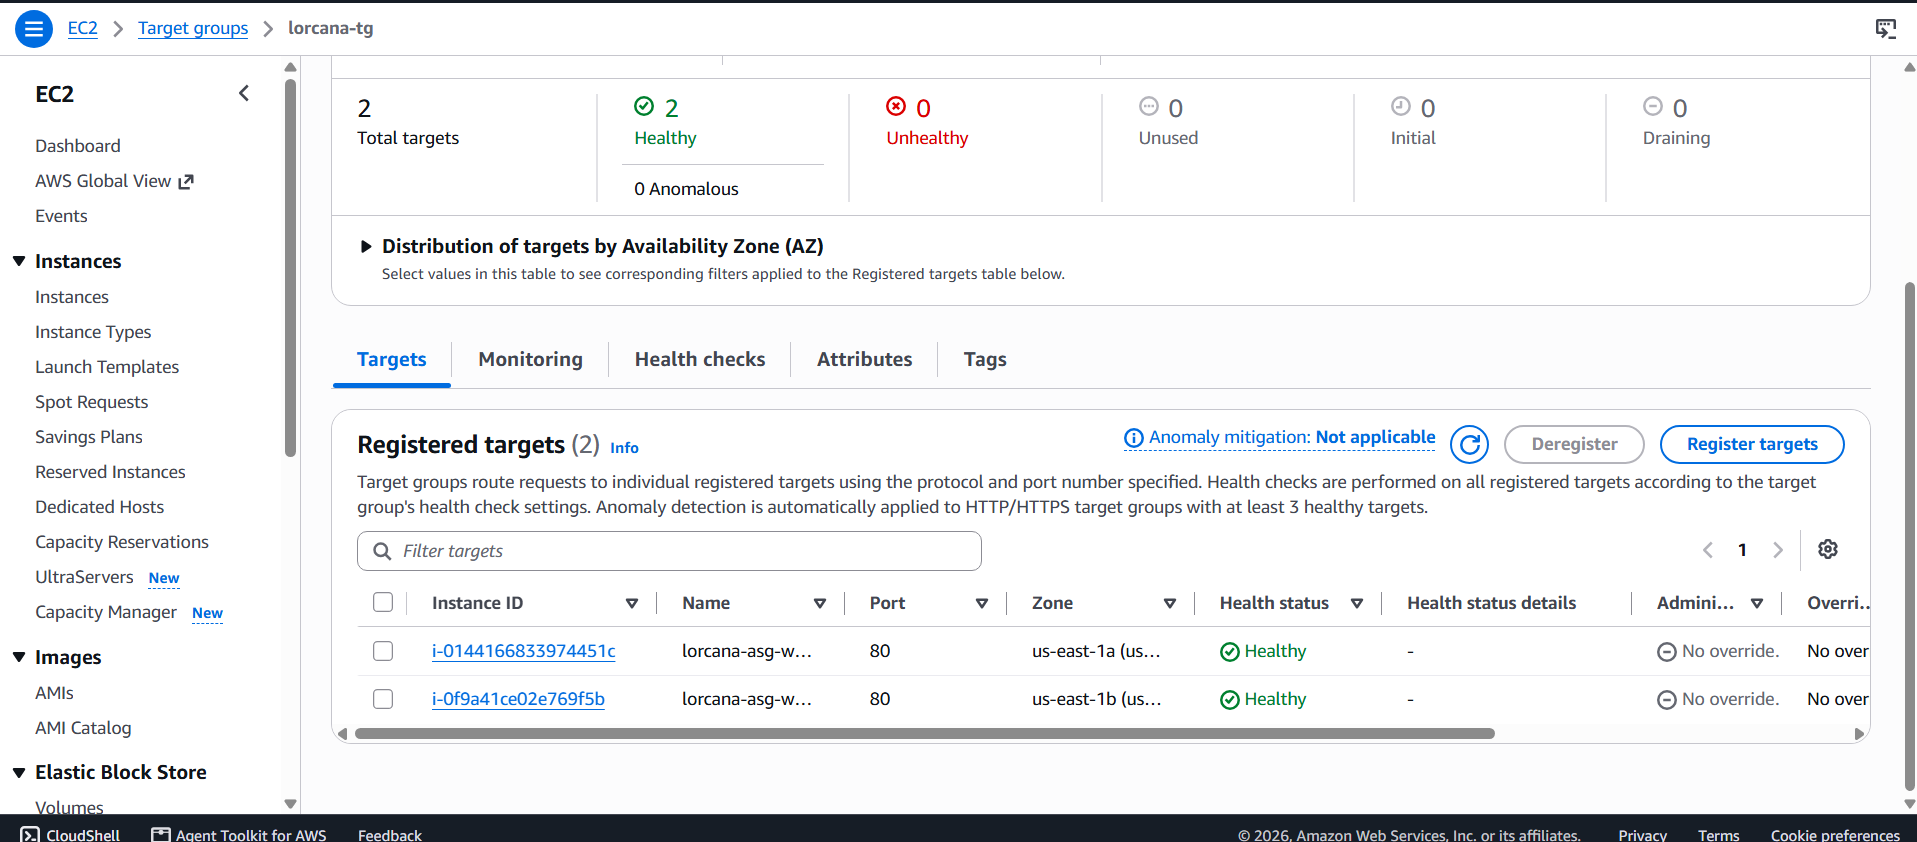
\includegraphics[width=\textwidth]{images/useindoc/aws_2026-10-12_target_group.png}
\caption{Target group \texttt{lorcana-tg} แท็บ Targets: 2 targets สถานะ Healthy 2 และ Unhealthy 0 เครื่องหนึ่งอยู่ใน \texttt{us-east-1a} และอีกเครื่องอยู่ใน \texttt{us-east-1b} พอร์ต 80}
\label{fig:aws_target_group}
\end{figure}

ภาพชุดนี้แสดงสถานะของ stack ขณะไม่มีโหลด จึงไม่มีภาพ alarm สั่งเพิ่มเครื่องจาก 2 เป็น 4 ผลการทดลองเรื่องการปรับจำนวนเครื่องตามโหลดอยู่ในไฟล์ข้อมูลของการทดลองเดิมใน \texttt{docs/01\_Reports/stage3\_evidence/} ซึ่งรันบน stack รุ่นก่อนหน้า
